\documentclass{article}

\usepackage{polski}
\usepackage{amsmath}
\usepackage{graphicx}
\usepackage{array}
\setlength{\extrarowheight}{.5ex}
\usepackage{float}
\usepackage{xcolor}

\newsavebox\MBox
\newcommand\Cline[2][red]{{\sbox\MBox{$#2$}%
  \rlap{\usebox\MBox}\color{#1}\rule[-1.2\dp\MBox]{\wd\MBox}{0.5pt}}}

\title{Sprawozdanie 1: Bramki i funkcje logiczne}
\author{\textbf{Jakub Szymczak, Damian Tworek,}\\ \textbf{Maksymilian Sulima, Łukasz Wala} \\
    \textit{AGH, Wydział Informatyki, Elektroniki i Telekomunikacji} \\
    \textit{Technika Cyfrowa 2021/2022}}
\date{Kraków, \today}

\begin{document}
\maketitle

\section{Ćwiczenie \textit{2a}}
Ideą ćwiczenia jest, na podstawie tabel prawdy, zaprojektować i praktycznie zrealizować asynchroniczny przerzutnik 
RS w oparciu o dwie bramki NAND, po czym jednoznacznie prztestować poprawność jego działania w programie Multisim.

\begin{figure}[H]
    \centering
    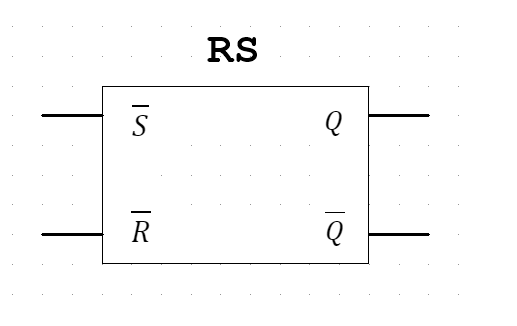
\includegraphics[width=\textwidth]{idea_1.png}
    \caption{Układ 2a}
\end{figure}

Zasada działania przerzutnika jest następująca: jeżeli na wejście $\overline{S}$ podanie zostana logiczne zero, wówczas
wymusi ona stan jeden na wyjściu $Q$ (stan "set"), natomiast logiczne zero na wejściu $\overline{R}$ wymusi zero na wyjściu $Q$ (stan "reset"). Przejście przerzutnika
do stanu neutralnego, gdzie na obu wejściach są jedynki, zachowuje poprzedni stan na wyjściu. Stan z dwoma zerami na wejściach
jest zabronionym, dla którego wyjście jest nieokreślone. Również przed pierwszą zmianą stanu stan jest nieokreślony.

\subsection{Rozwiązanie teoretyczne}
Rozpoczniemy od stworzenia tabeli przejść, gdzie $Q_{n-1}$ jest poprzednim stanem przerzutnika

\begin{table}[H]
    \centering
    \begin{tabular}{|l|l|l|l|}
    \hline
    $\overline{S}$ & $\overline{R}$ & Q & $\overline{Q}$ \\ \hline
    0 & 1 & 1 & 0 \\ \hline
    1 & 0 & 0 & 1 \\ \hline
    1 & 1 & $Q_{n-1}$ & $\overline{Q}_{n-1}$ \\ \hline
    0 & 0 & - & - \\ \hline
    \end{tabular}
    \caption{Tabela przejść}
\end{table}

Na podstawie tabeli 1 skonstruowana zostanie tabela Karnough dla $Q$

\begin{figure}[H]
    \centering
    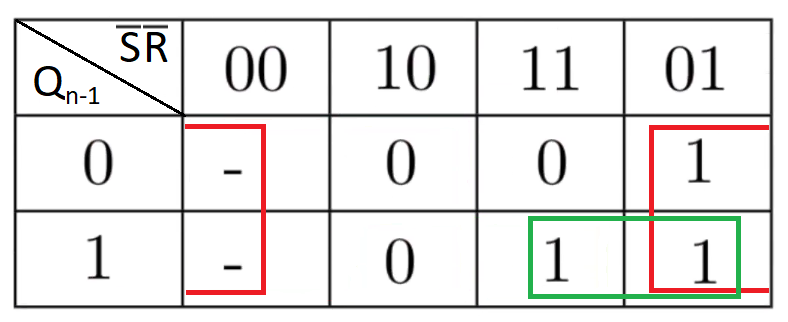
\includegraphics[width=\textwidth]{tab_kar_1.png}
    \caption{Tabela Karnough dla $Q$}
\end{figure}

Poniżej wzór na podstawie tabeli Karnough, z prawa podwójnej negacji

\[Q = \Cline[red]{\overline{\overline{S}}}+\Cline[green]{\overline{R}Q_{n-1}}=S+\overline{R}Q_{n-1}\]

Korzystając z prawa de Morgana

\[Q=\overline{\overline{S}\:\overline{\overline{R}Q_{n-1}}}\]

\begin{figure}[H]
    \centering
    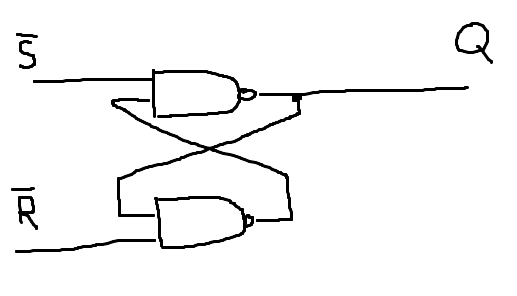
\includegraphics[width=\textwidth]{wypr_rs1.jpg}
    \caption{Projekt układu dla $Q$}
\end{figure}

Poniżej tabela Karnough dla $\overline{Q}$

\begin{figure}[H]
    \centering
    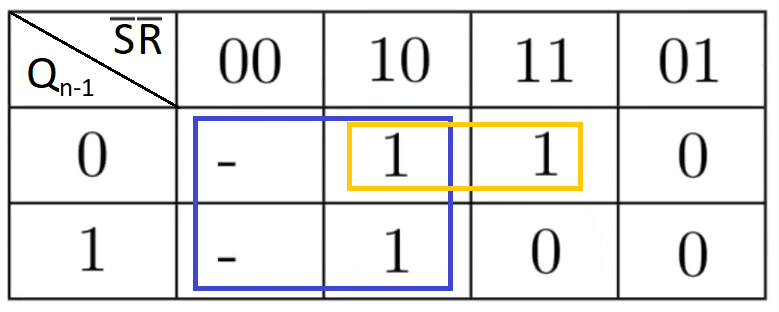
\includegraphics[width=\textwidth]{tab_kar_2.png}
    \caption{Tabela Kranough dla $\overline{Q}_{n}$}
\end{figure}

Poniżej wzór na podstawie tabeli Karnough dla $\overline{Q}_{n}$, z prawa podwójnej negacji

\[\overline{Q}=\Cline[blue]{\overline{\overline{R}}}+\Cline[yellow]{\overline{S}\:\overline{Q}_{n-1}}=R+\overline{S}\:\overline{Q}_{n-1}\]

Korzystając z prawa de Morgana

\[\overline{Q}=\overline{\overline{R}\:\overline{\overline{S}\:\overline{Q}_{n-1}}}\]

\begin{figure}[H]
    \centering
    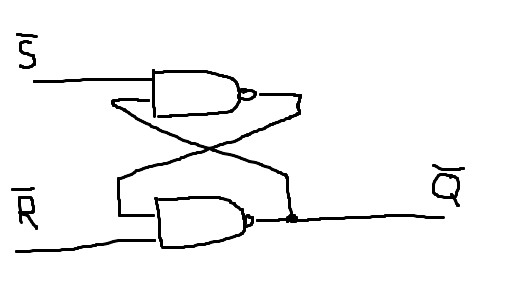
\includegraphics[width=\textwidth]{wypr_rs2.jpg}
    \caption{Projekt układu dla $\overline{Q}$}
\end{figure}

Można zauważyć, że układy te są symetryczne, więc można je połączyć, żeby otrzymać zarówno $Q$ oraz jego negację.

\begin{figure}[H]
    \centering
    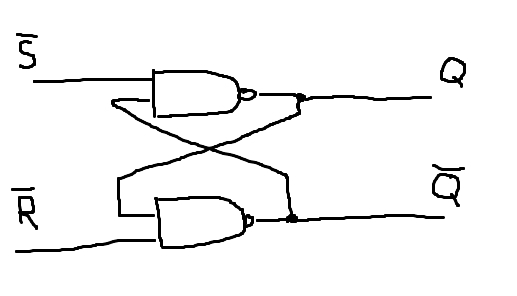
\includegraphics[width=\textwidth]{wypr_rs3.jpg}
    \caption{Projekt układu}
\end{figure}

\subsection{Implementacja w programie Multisim}
Poniżej implementacja układu w programie Multisim dla wszystkich możliwych stanów

\begin{figure}[H]
    \centering
    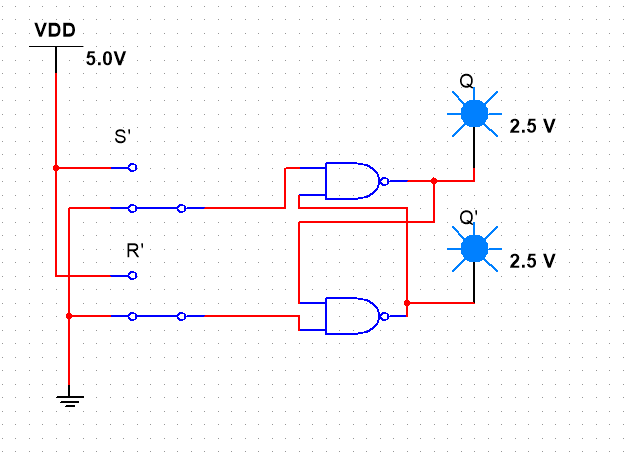
\includegraphics[width=0.8\textwidth]{rs_niokr.png}
    \caption{Układ w stanie nieokreślonym}
\end{figure}

\begin{figure}[H]
    \centering
    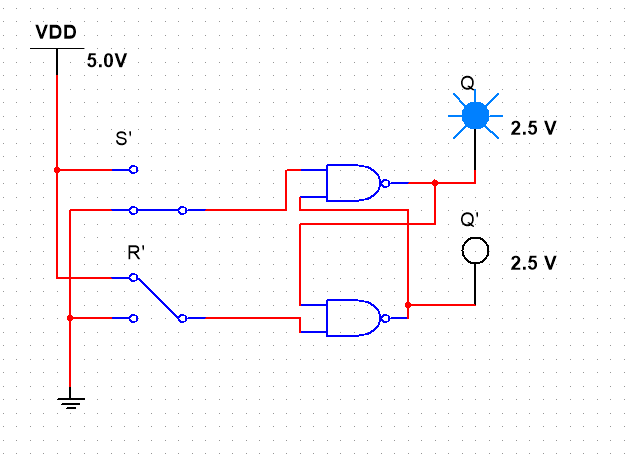
\includegraphics[width=0.8\textwidth]{rs_Q.png}
    \caption{Układ w stanie "set"}
\end{figure}

\begin{figure}[H]
    \centering
    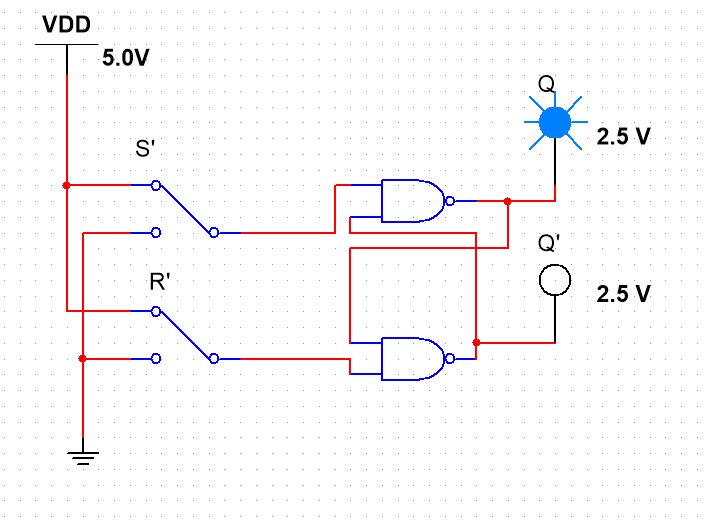
\includegraphics[width=0.8\textwidth]{rs_Q_save.png}
    \caption{Układ w stanie neutralnym, gdy w poprzednim był w stanie "set"}
\end{figure}

\begin{figure}[H]
    \centering
    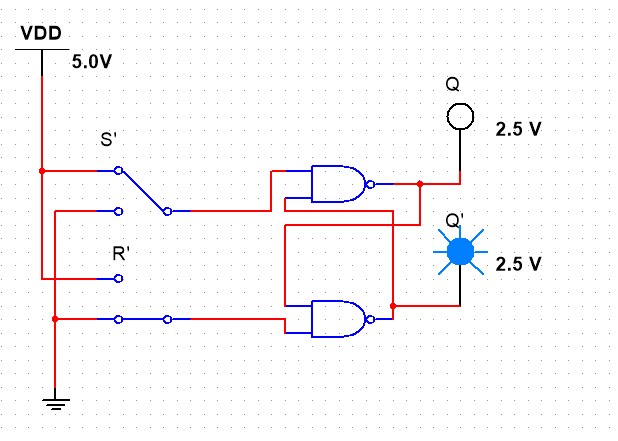
\includegraphics[width=0.8\textwidth]{rs_nQ.png}
    \caption{Układ w stanie "reset"}
\end{figure}

\begin{figure}[H]
    \centering
    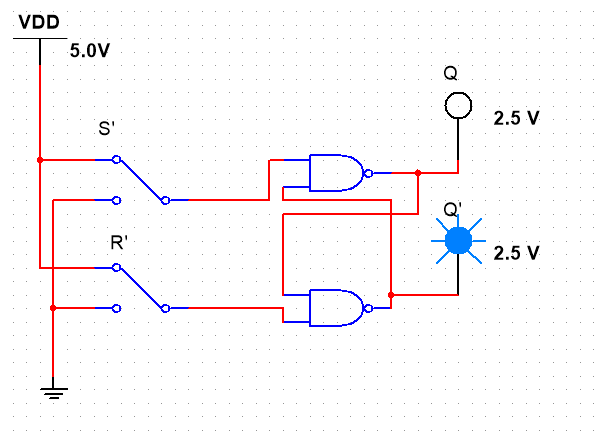
\includegraphics[width=0.8\textwidth]{rs_nQ_save.png}
    \caption{Układ w stanie neutralnym, gdy w poprzednim był w stanie "reset"}
\end{figure}

Poniżej automatyczny układ testujący dla przerzutnika RS:

\begin{figure}[H]
    \centering
    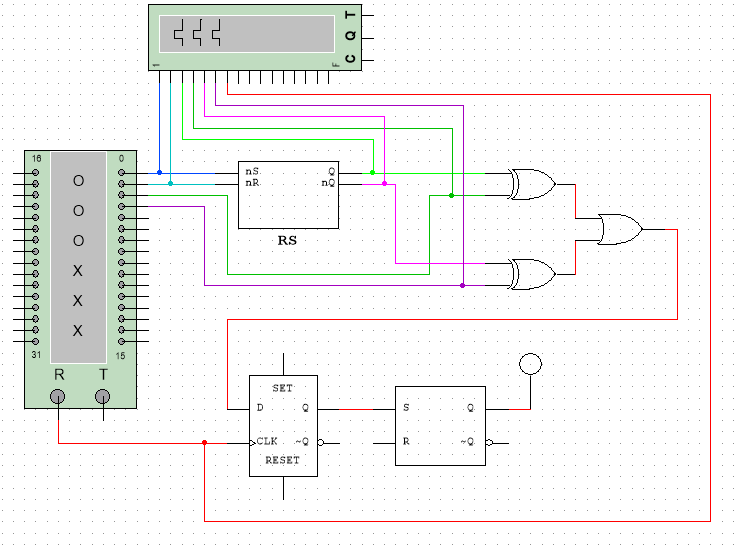
\includegraphics[width=\textwidth]{tester_1.png}
    \caption{Automatyczny układ testujący}
\end{figure}

\begin{figure}[H]
    \centering
    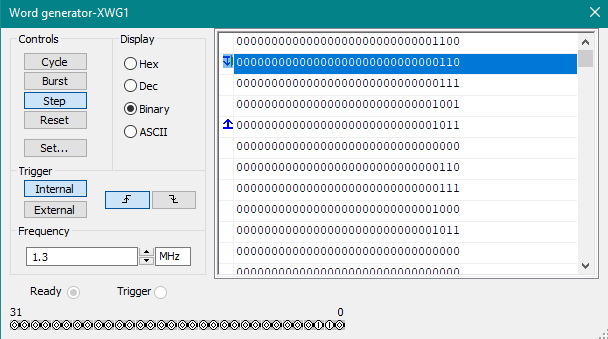
\includegraphics[width=\textwidth]{test_gen_1.png}
    \caption{Generator układu testującego}
\end{figure}

\begin{figure}[H]
    \centering
    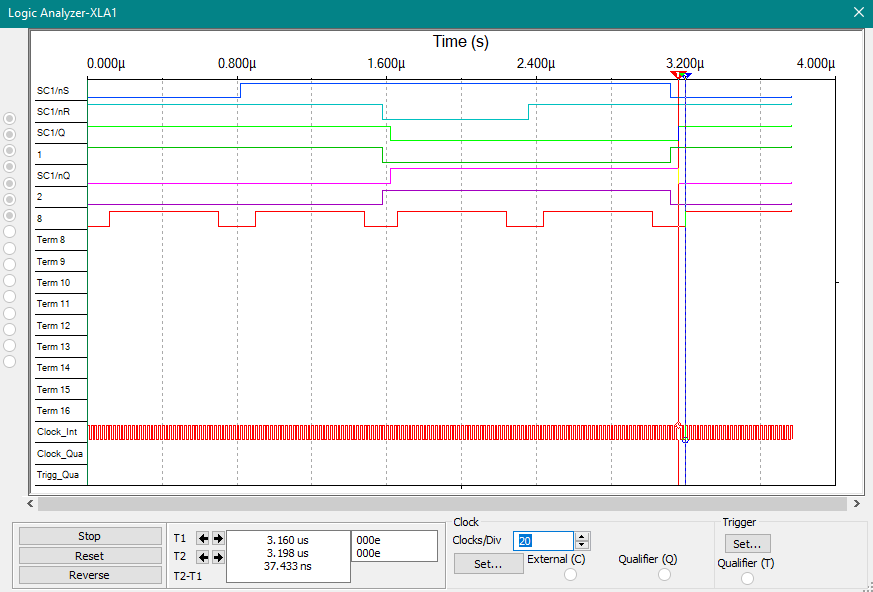
\includegraphics[width=\textwidth]{test_an_1.png}
    \caption{Analizator dla układu testującego}
\end{figure}

Generator słów na dwóch pierwszych bitach zawiera poszczególne możliwe wejścia do przerzutnika, natomiast na dwóch kolejnych
bitach są poprawne wyjścia, które są konfrontowane z wyjściami z przerzutnika przy pomocy bramek XOR. Ze względu na 
czas propagacji sygnału użyty został synchorniczny przerzutnik D, którego wejście CLK połączone jest z wyjściem R z generatora, które
mówi, że dane z generatora są gotowe, wówczas nie ma sytuacji, że moment zmiany wartości generatora zostanie odczytany jako
błąd testowanego przerzutnika. Do tego wykorzystano wbudowany do programu Multisim przerzutnik RS po to, żeby
po znalezionym błędzie lampka nie gasła.

\subsection{Wnioski}

\begin{itemize}
    \item
    Przrzutnik RS jest przerzutnikiem asynchronicznym, co czyni go podatnym na przypadkowe
    zmiany wejścia (na przykład spowodowane napięciem wyindukowanym na ścieżce czy przewodzie). Remedium na te
    problemy są przerzutniki synchroniczne, które zmieniają stan tylko w określonych momentach zmian stanów zegara. 

    \item
    Alternatywnym podejściem byłoby wyprowadzenie wzorów na podstawie tabeli Karnough zaznaczając grupy zer:
    \begin{figure}[H]
        \centering
        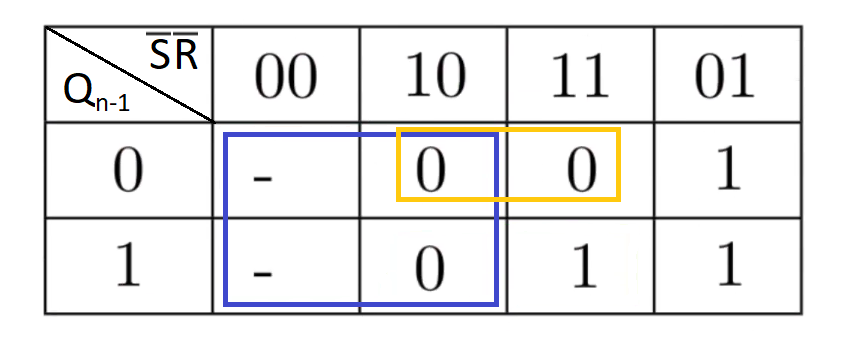
\includegraphics[width=\textwidth]{alt_tabela.png}
        \caption{Alternatywna tabela Karnough}
    \end{figure}
    Wówczas wzór wygląda następująco:
    \[Q=\Cline[blue]{\overline{\overline{R}}}\Cline[yellow]{(\overline{S}+\overline{Q}_{n-1})}=R(\overline{S}+\overline{Q}_{n-1})=
    R(\overline{\overline{\overline{S}}\:\overline{\overline{Q}}_{n-1}})=R(\overline{SQ_{n-1}})\]
    W tym przypadkie konieczne byłoby użycie więcej niż dwóch bramek NAND, co eliminuje to podejście.

    \item
    Podczas używania fizycznych przycisków w układach elektronicznych często może wystąpić efekt, gdzie metalowe styki
    odbijają się od siebie podczas przyciśnięcia i układ rejestruje kilka przyciśnięć zamiast jednego:

    \begin{figure}[H]
        \centering
        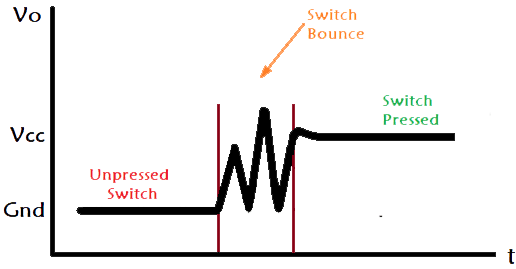
\includegraphics[width=0.8\textwidth]{bounce.png}
        \caption{Switch bounce}
    \end{figure}

    Asynchroniczny przerzutnik RS może posłużyć jako "debouncer" dla np. takiego przycisku w klawiaturze

    \begin{figure}[H]
        \centering
        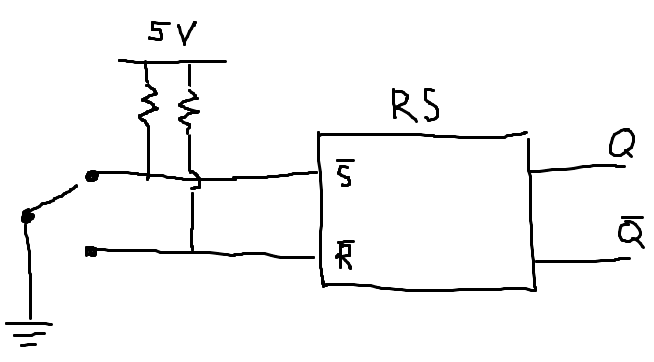
\includegraphics[width=0.8\textwidth]{debounce.png}
        \caption{Switch debouncer z użyciem przerzutnika RS}
    \end{figure}
    
\end{itemize}


\section{Ćwiczenie \textit{2b}}
Ideą ćwiczenia jest zbudowanie rejestru pierścieniowego. Powinien on realizować dwie podstawowe funkcje 
wybierane przy pomocy pojedynczego przełącznika trybu pracy:
\begin{itemize}
    \item
    powinien umożliwiać załadowanie do rejestru dowolnej ośmiobitowej wartości przy pomocy ośmiu przełączników,
    \item 
    powinien sprawić, że wpisana wcześniej wartość będzie w sposób ciągły krążyła w rejestrze. Np. skrajny bit z prawej strony
    powinien pojawić w następnym cyklu zegarowym na pierwszej pozycji z lewej strony.
\end{itemize}

\begin{figure}[H]
    \centering
    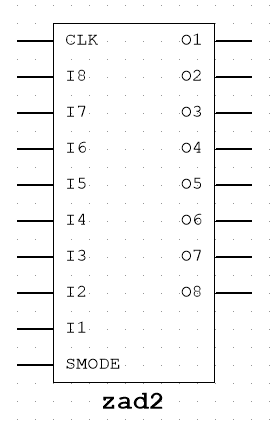
\includegraphics[width=0.5\textwidth]{idea_2.png}
    \caption{Układ 2b}
\end{figure}

\textbf{I1}...\textbf{I8} są wejściami, którymi można ustawić poszczególne bity, \textbf{O1}..\textbf{O8} to wyjścia, 
natomiast \textbf{CLK} to wejście zegara, \textbf{SMODE} to wejście włączające możliwość ustawiania wartości w rejestrze.

\subsection{Pomysł 1 - schemat koncepcyjny i implementacja}
Do zbudowania układu użyte zostaną przerzutnik typu \textbf{D} pokazane na poniższym rysunku. Przerzutnik typu D przepisuje stan
wejścia informacyjnego \textbf{D} na wyjście \textbf{Q}, przepisanie informacji następuje tylko przy odpowienim stanie wejścia zegarowego 
\textbf{CLK}, w tym przypadku przy zmianie jego stanu z 0 na 1. Dodatkowo wejścia \textbf{SET} oraz \textbf{RESET} działają analogicznie jak w przerzutniku RS.

\begin{figure}[H]
    \centering
    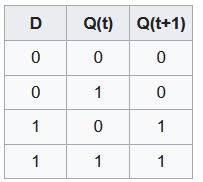
\includegraphics[width=0.5\textwidth]{przerzutnikD.png}
    \caption{Tabela przejść dla przerzutnika D}
\end{figure}

Układ bazowany na pierwszym pomyśle (udoskonalony w sekcjach "Pomysł 2") będzie się składał z ośmiu przerzutników D, gdzie wyjście \textbf{Q} przerzutnika poprzedniego połączone jest z wejściem
\textbf{D} przerzutnika kolejnego, natomiast ostatnie przerzutnik połączony jest z pierwszym. Tym sposobem przerzutniki będą przekazywać
sobie kolejne stany. Poniżej wycinek układu:


\begin{figure}[H]
    \centering
    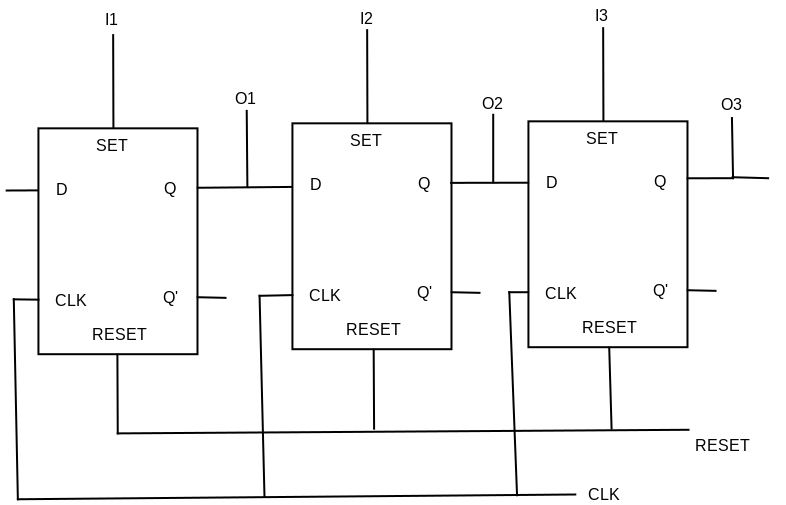
\includegraphics[width=\textwidth]{2_schemat.jpg}
    \caption{Schemat koncepcyjny pierwszej wersji układu 2b} 
\end{figure}

Załadowanie do rejestru początkowej wartości zostało zrealizowane za pomocą asynchornicznych wejść przerzutników D - 
\textbf{SET}. Do tego została również dodana możliwość resetowania wartości w rejestrze zrealizowana za pomocą wejść 
\textbf{RESET}.

Schemat zaimplementowany w programie Multisim wygląda następująco:

\begin{figure}[H]
    \centering
    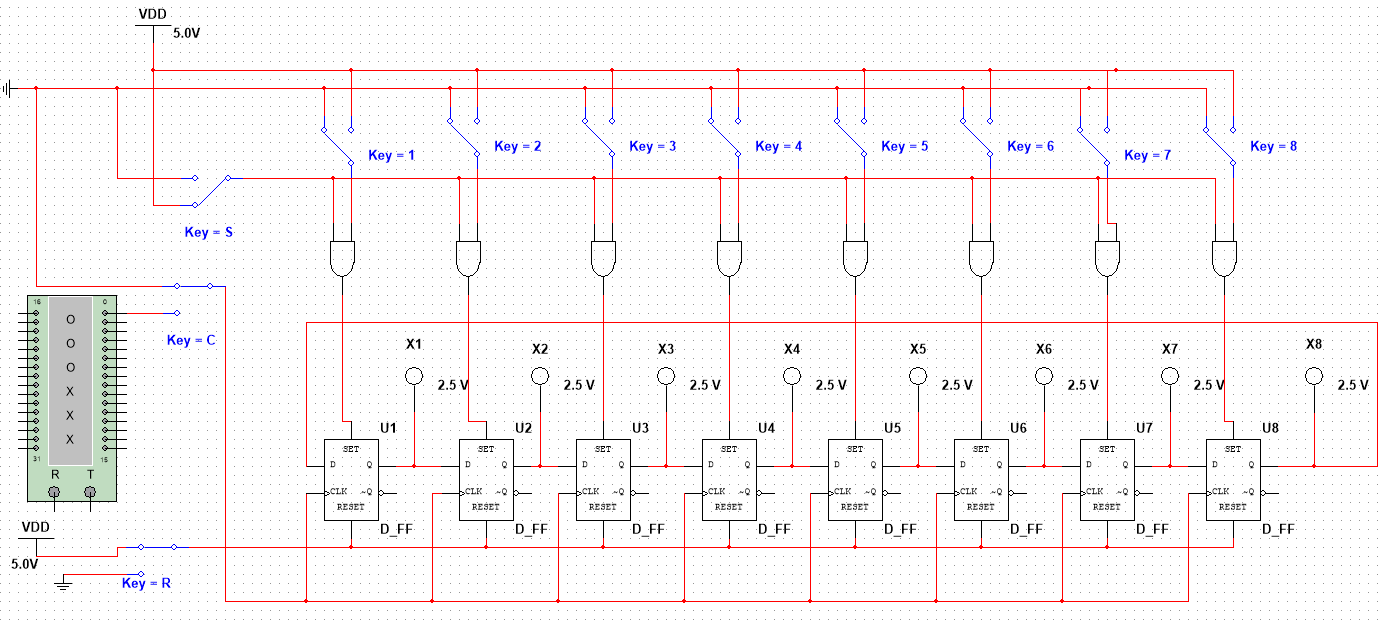
\includegraphics[width=\textwidth]{rej_1.png}
    \caption{Implementacja pierwszej wersji układu 2b}
\end{figure}

Rozwiązanie to jednak nie jest idealne - do ustawanie wartości w rejestrze wykorzystywane są operacje asynchroniczne,
które mogą być ryzykowne, lepsze rozwiązanie zaprezentowane jest w kolejnej sekcji.

\subsection{Pomysł 2 - schemat koncepcyjny i implementacja}
Drugi pomysł odrzuca używanie operacji asynchronicznych, natomiast do wprowadzania wartości do rejestru wykorzystuje
multipleksery w sposób zaprezentowany poniżej (również użyto przerzutników D).

\begin{figure}[H]
    \centering
    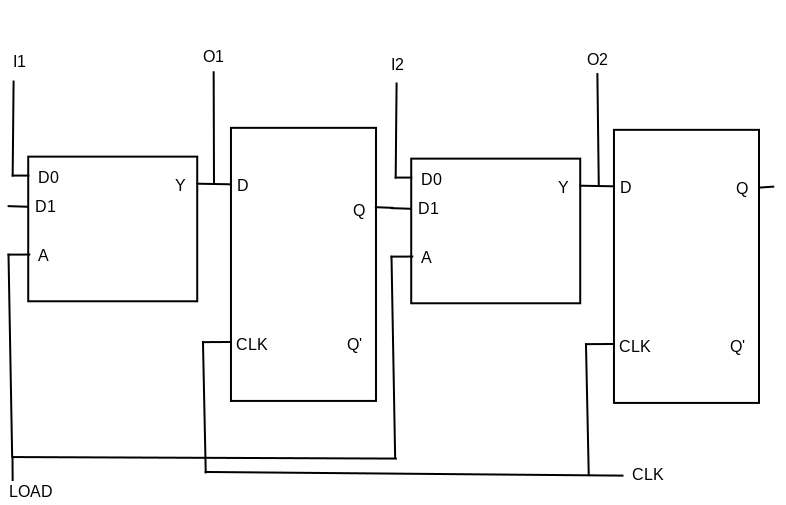
\includegraphics[width=\textwidth]{2_schemat_nowy.jpg}
    \caption{Schemat ulepszonej wersji układu 2b}
\end{figure}

Wejście \textbf{LOAD}, gdy ustawione na jedynkę logiczną, pozawala na załadowanie wartości do rejestru, w przeciwnym
wypadku pobierane są wartości z poprzedzającego multiplekser przerzutnika D.

Poniżej implementacja układu w programie Multisim:

\begin{figure}[H]
    \centering
    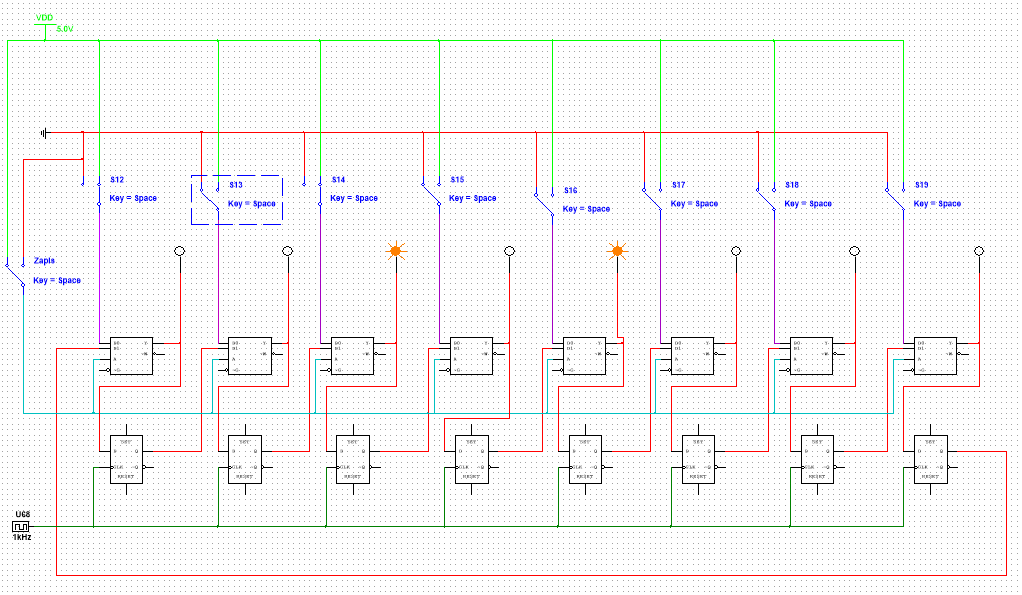
\includegraphics[width=\textwidth]{uklad_2_nowy.png}
    \caption{Implementacja ulepszonej wersji układu 2b}
\end{figure}

Poniżej automatyczny układ testujący

\begin{figure}[H]
    \centering
    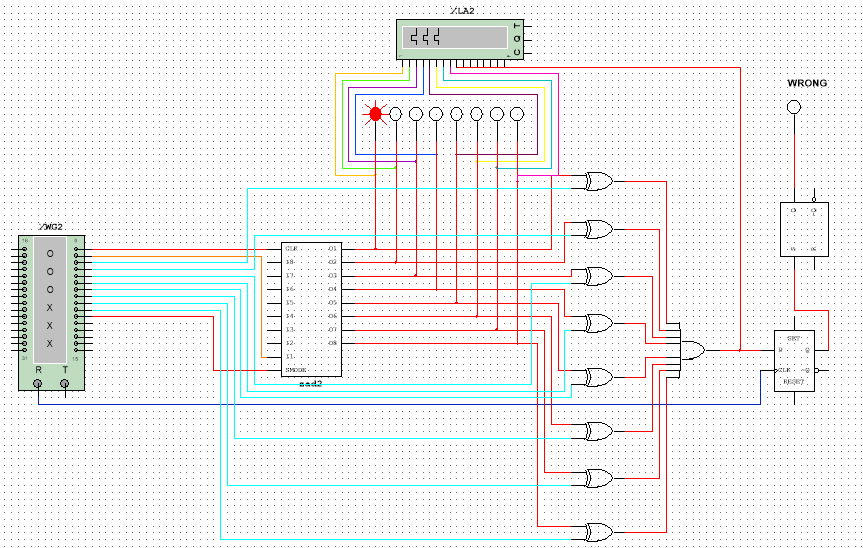
\includegraphics[width=\textwidth]{tester_2.png}
    \caption{Automatyczny układ testujący}
\end{figure}

\begin{figure}[H]
    \centering
    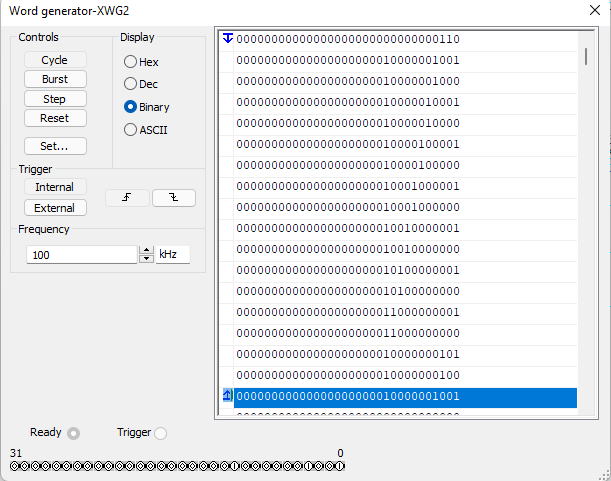
\includegraphics[width=\textwidth]{test_gen_2.png}
    \caption{Generator słów dla układu testującego}
\end{figure}

\begin{figure}[H]
    \centering
    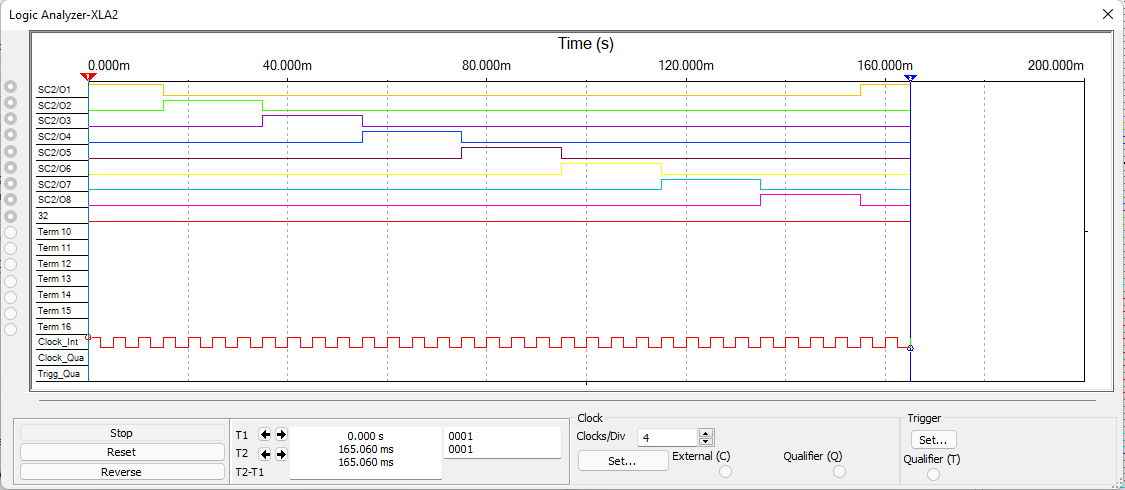
\includegraphics[width=\textwidth]{test_an_2.png}
    \caption{Analizator dla układu testującego}
\end{figure}

\subsection{Wnioski}
\begin{itemize}
    \item
    Alternatywnym podejściem byłoby zastosowanie innego rodzaju przerzutnika synchronicznego, np, przerzutnika
    JK. Przerzutnik JK może być łatwo przekonwertowany tak, żeby spełniał funckję przerzutnika D potrzebnego w 
    ćwiczeniu.
    \begin{figure}[H]
        \centering
        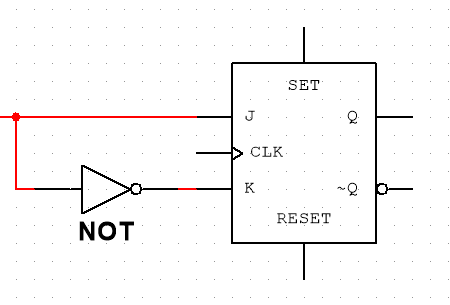
\includegraphics[width=0.7\textwidth]{jk_alt.png}
        \caption{Przerzutnik D stworzony przy pomocy przerzutnika JK}
    \end{figure}
    \item
    Rejestru pierścieniowego moża użyć jako urządzenia sterującego światłami choinkowymi. Np. niech co ósme światełko
    będzie przypięte do każdego wyjścia rejestru (1 wyjście do 1 światełka, 9 światełka, 17 światełka, 2 wyjście do
    2 światełka, 10 światełka itd.), wówczas można łatwo sterować sekwencjami światełek.
    \begin{figure}[H]
        \centering
        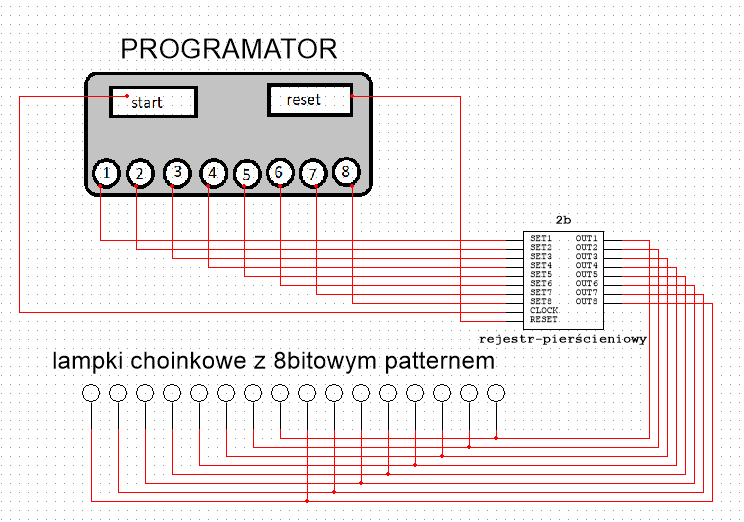
\includegraphics[width=0.8\textwidth]{choink.png}
        \caption{Światełka choinkowe}
    \end{figure}

\end{itemize}

\end{document}